\chapter{Natural transformations}
\label{chap:naturals}

\epigraph{
  ... and \emph{functor} has been defined in order to be able to
  define \emph{natural transformation}.
}{---\textcite[18]{maclane-1998}}

In this chapter we explore natural transformations and their relation
to polymorphic functions in Haskell and Agda.

\section{Introduction}
\label{sec:naturals-introduction}

Despite their name, natural transformations might be a first stumbling
block in the study of category theory. Just like functors are
morphisms of categories, natural transformations are morphisms of
functors, that is, morphisms of morphisms of categories. Besides,
examples tend to raise the level of mathematical sophistication
\parencites[433]{poigne-1992}[page 47]{rydeheard-1988}.

However, natural transformations are indeed natural, especially
natural transformations in functional programming. It is typical to
explain this idea with examples of parametrically polymorphic
functions such as appending an element to a list, extracting the first
component of a pair, reversing a list, etcetera.

One such function is the \texthaskell{head} function, which extracts
the first element of a list, whose type signature in Haskell
is\footnote{This is different from the standard \texthaskell{head}
  function.}
\begin{equation*}
  \text{\texthaskell{head :: [a] -> Maybe a}}
  \text{,}
\end{equation*}
and which is defined by the equations in Figure \ref{fig:head}.
\begin{figure}[htb]
  \begin{codehaskell}
                        head []    = Nothing
                        head (x:_) = Just x
  \end{codehaskell}
  \caption{The \texthaskell{head} function.}
  \label{fig:head}
\end{figure}
This is not any function, but a function of functors. Specifically, it
is a function from the \texthaskell{[]} functor to the
\texthaskell{Maybe} functor. Moreover, it is not just a function, but
rather a family of functions
\begin{equation*}
  \{
  \text{\texthaskell{head :: [a] -> Maybe a}}
    \mid \text{\texthaskell{a}} \in \catO{\hask}
  \}
\end{equation*}
indexed by the set of objects \catO{\hask}. In this case, it is
clearer to write, using the \texthaskell{ExplicitForAll} language
option,
\begin{equation*}
  \text{\texthaskell{head :: forall a. [a] -> Maybe a}}
\end{equation*}
for the type signature of the function.

The \texthaskell{head} function is natural or uniform in the sense
that, given two types \texthaskell{a} and \texthaskell{b}, a function
\texthaskell{f :: a -> b}, and a list of elements of \texthaskell{a},
mapping the function over the list and then extracting the first
element of the result is the same as extracting the first element of
the list and then mapping the function over the result. That is to
say,
\begin{equation*}
  \text{\texthaskell{head . fmap f = fmap f . head}}
  \text{,}
\end{equation*}
or, explicitly,
\begin{align*}
  &\text{\texthaskell{(head :: [b] -> Maybe b) . (fmap f :: [a] -> [b])}}\\
  &\text{\texthaskell{  =}}\\
  &\text{\texthaskell{(fmap f :: Maybe a -> Maybe b) . (head :: [a] -> Maybe a)}}
  \text{,}
\end{align*}
which is the commutativity of the diagram in Figure
\ref{fig:naturality-head}.
\begin{figure}[htb]
  \begin{center}
    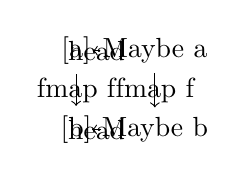
\begin{tikzpicture}
      \node (f a)                {\texthaskell{[a]}};
      \node (f b) [below of=f a] {\texthaskell{[b]}};
      \node (g a) [right of=f a] {\texthaskell{Maybe a}};
      \node (g b) [below of=g a] {\texthaskell{Maybe b}};

      \draw [->] (f a) to node [swap] {\texthaskell{fmap f}} (f b);
      \draw [->] (g a) to node        {\texthaskell{fmap f}} (g b);

      \draw [->] (f a) to node        {\texthaskell{head}} (g a);
      \draw [->] (f b) to node [swap] {\texthaskell{head}} (g b);
    \end{tikzpicture}
  \end{center}
  \caption{Naturality of the \texthaskell{head} function.}
  \label{fig:naturality-head}
\end{figure}

Even if this is an intuitive property of the \texthaskell{head}
function and proving it is quite simple, it says a lot about its
behavior and the behavior of all the functions that are part of the
family that it defines.

All of these facts about the \texthaskell{head} function and other
parametrically polymorphic functions are abstracted by natural
transformations, which will be explored in this chapter.

\section{Natural transformations}
\label{sec:naturals}

``The trinity of concepts category, functor, and natural
transformation is what category theory is built on''
\parencite{nlab-category-theory}.

\begin{definition}
  \label{def:natural}

  %% \parencites[16]{maclane-1998}[435--436]{poigne-1992}

  Let $\func{F}: \cat{C} \to \cat{D}$ and $\func{G}: \cat{C} \to
  \cat{D}$ be functors\footnote{Whenever a functor $\func{F}: \cat{C}
    \to \cat{D}$ is mentioned, its object and morphism functions
    (\funcO{F} and \funcM{F}, respectively) are implicitly mentioned
    as well. See Definition \ref{def:functor}.} for categories \cat{C}
  and \cat{D}. A natural transformation
  \begin{equation}
    \label{eq:natural}
    \nat{\tau}: \func{F} \to \func{G}: \cat{C} \to \cat{D}
  \end{equation}
  is a function
  \begin{equation}
    \label{eq:natural-transformation}
    \nat{\tau}: \catO{C} \to \catM{D}
  \end{equation}
  which assigns to each object $a \in \catO{C}$ a morphism
  \begin{equation*}
    \natO{\tau}{a}: \funcO{F}(a) \to \funcO{G}(a) \in \catM{D}
    \text{,}
  \end{equation*}
  called a component of the natural transformation, such that, for all
  morphisms $f: a \to b \in \catM{C}$,
  \begin{equation}
    \label{eq:naturality}
    \natO{\tau}{b} \comp \funcM{F}(f) = \funcM{G}(f) \comp \natO{\tau}{a}
    \text{,}
  \end{equation}
  called naturality of the natural transformation, that is, such that
  the diagram in Figure \ref{fig:naturality} is commutative.

  \begin{figure}[htbp]
    \begin{center}
      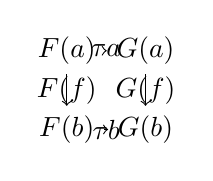
\begin{tikzpicture}
        \node (f a)                {$\funcO{F}(a)$};
        \node (f b) [below of=f a] {$\funcO{F}(b)$};
        \node (g a) [right of=f a] {$\funcO{G}(a)$};
        \node (g b) [below of=g a] {$\funcO{G}(b)$};

        \draw [->] (f a) to node [swap] {$\funcM{F}(f)$} (f b);
        \draw [->] (g a) to node        {$\funcM{G}(f)$} (g b);

        \draw [->] (f a) to node        {$\natO{\tau}{a}$} (g a);
        \draw [->] (f b) to node [swap] {$\natO{\tau}{b}$} (g b);
      \end{tikzpicture}
    \end{center}
    \caption{Naturality of a natural transformation.}
    \label{fig:naturality}
  \end{figure}

  Equivalently, a natural transformation \eqref{eq:natural} is a set
  of morphisms of \catM{D}
  \begin{equation}
    \nat{\tau} = \{\natO{\tau}{a}: \funcO{F}(a) \to \funcO{G}(a) \in
    \catM{D} \mid a \in \catO{C}\}
  \end{equation}
  indexed by the set of objects \catO{C} such that
  \eqref{eq:naturality} holds.

\end{definition}

\begin{remark}
  \label{re:natural-translation}

  %% Since \func{F} sends objects and morphisms of \cat{C} to objects and
  %% morphisms of \cat{D}, it may thought of as giving a picture of
  %% \cat{C} in \cat{D} \parencites[16]{maclane-1998}[10]{marquis-2013}.

  Since a functor $\func{F}: \cat{C} \to \cat{D}$ may be thought of as
  a picture of all the objects and morphisms of \cat{C} in \cat{D} , a
  natural transformation $\nat{\tau}: \func{F} \to \func{G}: \cat{C}
  \to \cat{D}$ may be thought of as a mapping or translation from the
  picture \func{F} into the picture \func{G} with all diagrams like
  that of Figure \ref{fig:natural-translation} commutative
  \parencite[16]{maclane-1998}. This gives a better idea of a natural
  transformation as a morphism of functors.
  \begin{figure}[htbp]
    \begin{center}
      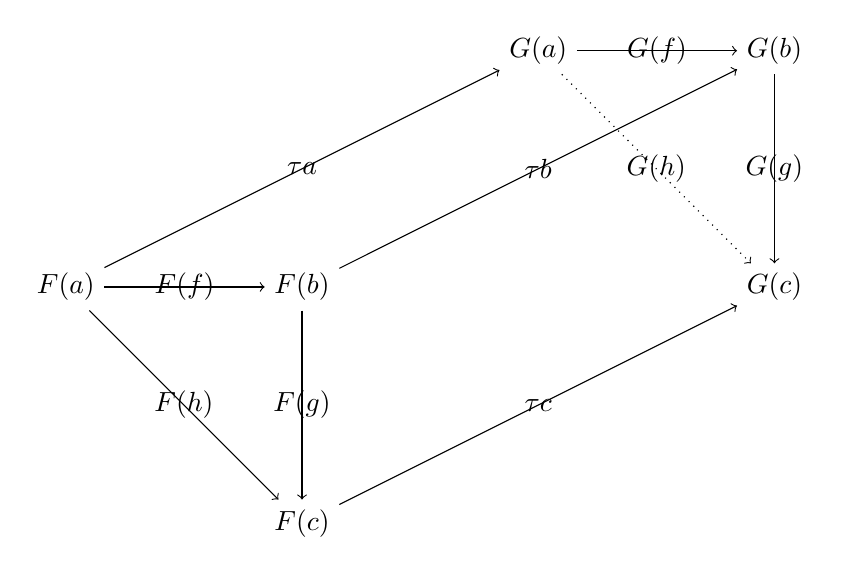
\begin{tikzpicture}[node distance=3cm]
        \node (f a)              {$\funcO{F}(a)$};
        \node (f b) [right of=f a] {$\funcO{F}(b)$};
        \node (f c) [below of=f b] {$\funcO{F}(c)$};

        \draw [->] (f a) to node        {$\funcM{F}(f)$} (f b);
        \draw [->] (f b) to node        {$\funcM{F}(g)$} (f c);
        \draw [->] (f a) to node [swap] {$\funcM{F}(h)$} (f c);

        \node (g a) [right of=f b,above of=f b] {$\funcO{G}(a)$};
        \node (g b) [right of=g a]              {$\funcO{G}(b)$};
        \node (g c) [below of=g b]              {$\funcO{G}(c)$};

        \draw [->] (g a) to node        {$\funcM{G}(f)$} (g b);
        \draw [->] (g b) to node        {$\funcM{G}(g)$} (g c);
        \draw [dotted,->] (g a) to node [swap] {$\funcM{G}(h)$} (g c);

        \draw [->] (f a) to node {$\natO{\tau}{a}$} (g a);
        \draw [->] (f b) to node {$\natO{\tau}{b}$} (g b);
        \draw [->] (f c) to node {$\natO{\tau}{c}$} (g c);
      \end{tikzpicture}
    \end{center}
    \caption{Natural transformations are morphisms of functors.}
    \label{fig:natural-translation}
  \end{figure}

\end{remark}

\begin{remark}
  \label{re:category-functor-natural}

  According to \textcite[18]{maclane-1998}, ``\emph{category} has been
  defined in order to be able to define \emph{functor} and
  \emph{functor} has been defined in order to be able to define
  \emph{natural transformation}.'' Originally (that is, in
  \parencite{eilenberg-maclane-1942,eilenberg-maclane-1945}), this meant that categories
  and functors were dispensable. However, in this context (which is
  the context implied by the epigraphs of Chapters \ref{chap:functors}
  and \ref{chap:naturals}), this also means that the study of functors
  is not complete without the study of natural transformations. In
  other words, \parencite{eilenberg-maclane-1942} does not define categories and
  functors because of their generality. These concepts were implicit.
  \todo{Rewrite this remark.}

\end{remark}

\begin{remark}[Why is a natural transformation \emph{natural}?]
  \label{re:natural}

  Given two functors \func{F} and \func{G} from \cat{C} to \cat{D},
  all objects $\funcO{F}(a)$ and morphisms $\funcM{F}(f)$ are somewhat
  \emph{structured} by \func{F}. Natural transformations allow to talk
  about transformations between such structures generically,
  \emph{natural} meaning \emph{uniform} \parencite[page
    77]{elkins-2009}. According to \parencite[page 30]{maclane-1998},
  the word \emph{natural} was taken from then (1940s) current informal
  parlance. And, in \parencite{maclane-2005}, the author says that
  \emph{natural} meant that natural transformations behave correctly
  or well for maps, and that it follows informal terminology used for
  such commutativity behavior. Another way of thinking about the word
  \emph{natural} is that natural transformations are defined by first
  principles, independently of any choice.

\end{remark}

\begin{example}
  \label{ex:natural-identity}

  Given a category \cat{C}, its identity function\footnote{See
    Definition \ref{def:category}.}
  \begin{equation*}
    \id: \catO{C} \to \catM{C}
    \text{,}
  \end{equation*}
  which assigns to each object $a \in \catO{C}$ a morphism
  \begin{equation*}
    \idO{a}: a \to a \in \catM{C}
    \text{,}
  \end{equation*}
  is a natural transformation\footnote{See Example
    \ref{ex:functor-identity}.}
  \begin{equation*}
    \id: \func{I} \to \func{I}: \cat{C} \to \cat{C}
    \text{.}
  \end{equation*}

  \begin{proof}

    For all morphisms $f: a \to b \in \catM{C}$, the naturality of the
    identity natural transformation is given by
    \begin{equation*}
      \idO{b} \comp f = f \comp \idO{a}
      \text{,}
    \end{equation*}
    or, equivalently, by the commutativity of the diagram in Figure
    \ref{fig:natural-id-a} (or by the commutativity of the diagram in
    Figure \ref{fig:natural-id-b}, which makes explicit the functors
    involved), which holds by \eqref{eq:category-identity}.

    \begin{figure}[htbp]
      \begin{subfigure}[b]{0.5\linewidth}
        \begin{center}
          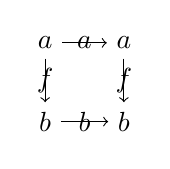
\begin{tikzpicture}
            \node (f a)                {$a$};
            \node (f b) [below of=f a] {$b$};
            \node (g a) [right of=f a] {$a$};
            \node (g b) [below of=g a] {$b$};

            \draw [->] (f a) to node [swap] {$f$} (f b);
            \draw [->] (g a) to node        {$f$} (g b);

            \draw [->] (f a) to node        {$\idO{a}$} (g a);
            \draw [->] (f b) to node [swap] {$\idO{b}$} (g b);
          \end{tikzpicture}
        \end{center}
        \caption{}
        \label{fig:natural-id-a}
      \end{subfigure}
      \begin{subfigure}[b]{0.5\linewidth}
        \begin{center}
          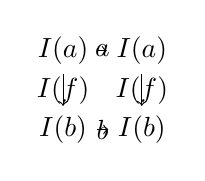
\begin{tikzpicture}
            \node (f a)                {$\funcO{I}(a)$};
            \node (f b) [below of=f a] {$\funcO{I}(b)$};
            \node (g a) [right of=f a] {$\funcO{I}(a)$};
            \node (g b) [below of=g a] {$\funcO{I}(b)$};

            \draw [->] (f a) to node [swap] {$\funcM{I}(f)$} (f b);
            \draw [->] (g a) to node        {$\funcM{I}(f)$} (g b);

            \draw [->] (f a) to node        {$\idO{a}$} (g a);
            \draw [->] (f b) to node [swap] {$\idO{b}$} (g b);
          \end{tikzpicture}
        \end{center}
        \caption{}
        \label{fig:natural-id-b}
      \end{subfigure}
      \caption{Naturality of the identity natural transformation.}
      \label{fig:natural-id}
    \end{figure}

  \end{proof}

\end{example}

\begin{example}
  \label{ex:natural-identity-power-set}

  %% \parencite[11]{marquis-2013}

  It is possible, and natural, to define a translation from the
  identity functor (see Example \ref{ex:functor-identity}) into the power
  set functor (see Example \ref{ex:functor-power-set}). Indeed, the
  function
  \begin{equation*}
    \nat{\eta}: \catO{\set} \to \catM{\set}
    \text{,}
  \end{equation*}
  which assigns to each set $X \in \catO{\set}$ a function
  \begin{equation*}
    \natO{\eta}{X}: \funcO{I}(X) \to \funcO{P}(X) \in \catM{\set}
  \end{equation*}
  such that, for all $x \in X$,
  \begin{equation}
    \label{eq:eta}
    \natO{\eta}{X}(x) = \{x\}
    \text{,}
  \end{equation}
  is a natural transformation
  \begin{equation*}
    \nat{\eta}: \func{I} \to \func{P}: \set \to \set
    \text{.}
  \end{equation*}

  \begin{proof}

    Given a function $f: X \to Y \in \catM{\set}$ and an element $x
    \in X$,
    \begin{steps}
      \step{$(\natO{\eta}{Y} \comp \funcM{I}(f))(x)$}\label{eta-a}
        \eqbydef{\comp}
      \step{$\natO{\eta}{Y}(\funcM{I}(f)(x))$}
        \eqbydef{\funcM{I} \eqref{eq:functor-identity-morphism}}
      \step{$\natO{\eta}{Y}(f(x))$}
        \eqbydef{\nat{\eta} \eqref{eq:eta}}
      \step{$\{f(x)\}$}
        \eqbydef{\funcM{P} \eqref{eq:functor-power-set-morphism}}
      \step{$\funcM{P}(f)(\{x\})$}
        \eqbydef{\nat{\eta} \eqref{eq:eta}}
      \step{$\funcM{P}(f)(\natO{\eta}{X}(x))$}
        \eqbydef{\comp}
      \step{$(\funcM{P}(f) \comp \natO{\eta}{X})(x)$.}\label{eta-b}
    \end{steps}
    Then, by steps \ref{eta-a}--\ref{eta-b},
    \begin{steps}[resume]
      \step{$\natO{\eta}{Y} \comp \funcM{I}(f) = \funcM{P}(f) \comp
        \natO{\eta}{X}$,}
    \end{steps}
    which is the naturality of \nat{\eta}, or, equivalently, the
    commutativity of the diagram in Figure \ref{fig:naturality-eta}.

    \begin{figure}[htbp]
      \begin{center}
        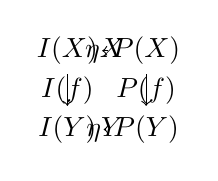
\begin{tikzpicture}
          \node (f a)                {$\funcO{I}(X)$};
          \node (f b) [below of=f a] {$\funcO{I}(Y)$};
          \node (g a) [right of=f a] {$\funcO{P}(X)$};
          \node (g b) [below of=g a] {$\funcO{P}(Y)$};

          \draw [->] (f a) to node [swap] {$\funcM{I}(f)$} (f b);
          \draw [->] (g a) to node        {$\funcM{P}(f)$} (g b);

          \draw [->] (f a) to node        {$\natO{\eta}{X}$} (g a);
          \draw [->] (f b) to node [swap] {$\natO{\eta}{Y}$} (g b);
        \end{tikzpicture}
      \end{center}
      \caption{Naturality of $\eta$ (Example \ref{ex:natural-identity-power-set}).}
      \label{fig:naturality-eta}
    \end{figure}

  \end{proof}

\end{example}

\section{Natural transformations in Haskell}
\label{sec:naturals-haskell}

\todo{This used to be a section called Polymorphic functions.}

As mentioned in Section \ref{sec:naturals-introduction}, polymorphic
functions in functional programming correspond to natural
transformations. This statement is based on, for instance,
\parencites[34]{bird-demoor-1997}[78]{elkins-2009}[435, 436]{poigne-1992}[48,
  49]{rydeheard-1986}[113]{rydeheard-1988}[350]{wadler-1989}.

The kind of polymorphism that the statement above refers to is
\emph{parametric polymorphism}
\parencite[following][37]{strachey-2000} or \emph{universal parametric
  polymorphism} \parencite[following][4]{cardelli-1985}. A polymorphic
function is a function whose parameters can have more than one type. A
parametrically polymorphic function works uniformly in a range of
types and this uniformity is achieved by type parameters. It is also a
generic function \parencite[4, 5]{cardelli-1985}.

Polymorphic functions can be thought of as functions of functors in order
to relate them to natural transformations (see Definition \ref{def:natural}).
In fact, given two functors \texthaskell{f} and \texthaskell{g}, a
natural transformation \texthaskell{tau} is a polymorphic function
\begin{equation}
  \label{eq:natural-haskell-a}
  \text{\texthaskell{tau :: f a -> g a}}
\end{equation}
such that, for all functions \texthaskell{f :: a -> b},
\begin{equation}
  \label{eq:naturality-haskell}
  \text{\texthaskell{tau . fmap f = fmap f . tau}}
  \text{,}
\end{equation}
that is, such that the diagram in Figure \ref{fig:naturality-haskell}
is commutative. An intuitive idea behind naturality is that terms
evaluated in related environments yield related values
\parencite[347--348]{wadler-1989}.
\begin{figure}[htbp]
  \begin{center}
    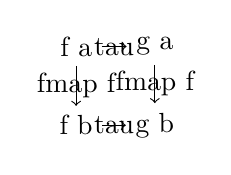
\begin{tikzpicture}
      \node (f a)                {\texthaskell{f a}};
      \node (f b) [below of=f a] {\texthaskell{f b}};
      \node (g a) [right of=f a] {\texthaskell{g a}};
      \node (g b) [below of=g a] {\texthaskell{g b}};

      \draw [->] (f a) to node [swap] {\texthaskell{fmap f}} (f b);
      \draw [->] (g a) to node        {\texthaskell{fmap f}} (g b);

      \draw [->] (f a) to node        {\texthaskell{tau}} (g a);
      \draw [->] (f b) to node [swap] {\texthaskell{tau}} (g b);
    \end{tikzpicture}
  \end{center}
  \caption{Naturality in Haskell \eqref{eq:naturality-haskell}.}
  \label{fig:naturality-haskell}
\end{figure}

The type of the polymorphic function \texthaskell{tau}
\eqref{eq:natural-haskell-a} could be written as
\begin{equation}
  \label{eq:natural-haskell-b}
  \text{\texthaskell{tau :: forall a. f a -> g a}}
  \text{,}
\end{equation}
which makes it easier to think about it as set of functions indexed
by the set of objects \catO{\hask}, that is,
\begin{equation*}
  \text{\texthaskell{tau}} =
  \{\text{\texthaskell{tau :: f a -> g a}} \mid \text{\texthaskell{a}}
  \in \catO{\hask}\}
  \text{.}
\end{equation*}

Naturality in Haskell is the ``theorem for free'' of
\parencite{wadler-1989}. Given the type of a polymorphic function, it
is possible to conclude that it satisfies its naturality
\eqref{eq:naturality-haskell}. This result is known as
\emph{parametricity} due to its relation with parametric polymorphism.

Parametricity is a reformulation of Reynold's abstraction theorem and
is also known as the representation theorem. A different approach to
that of \parencite{wadler-1989} is the one in \parencite{abadi-1993}.

Even though \parencite[page 350]{wadler-1989} says that parametricity
can be expressed more concisely in terms of lax natural
transformations, neither it nor \parencite{abadi-1993} study natural
transformations and their relation to polymorphic functions.

The relation between natural transformations and parametrically
polymorphic functions is not as straightforward as discussed here.
Polymorphic functions actually correspond to lax natural
transformations, but this fact is beyond the scope of this
dissertation.

Finally, it is important to note that parametricity guarantees that a
polymorphic function satisfies its naturality, but it does not provide
a proof of it. Parametricity does not require the definition of a
function (only its type), but proving naturality does.

\begin{example}
  \label{ex:natural-identity-haskell}

  The identity function of \hask
  \begin{equation*}
    \text{\texthaskell{id :: a -> a}}
  \end{equation*}
  is a natural transformation.

  \begin{proof}

    Example \ref{ex:natural-identity} establishes that the identity
    function is a natural transformation regardless of which category
    it belongs to. For that reason, the identity function of \hask is
    a natural transformation. Equivalently, \eqref{eq:hask-identity}
    in Section \ref{sec:category-haskell} means that naturality holds
    for \texthaskell{id}.

  \end{proof}

\end{example}

\begin{example}
  \label{ex:natural-head-haskell}

  The \texthaskell{head} function, which extracts the first element of
  a list, is a natural transformation from the \texthaskell{[]}
  functor into the \texthaskell{Maybe} functor.
  \begin{codehaskell}
    head :: [a] -> Maybe a
    head []    = Nothing
    head (x:_) = Just x
  \end{codehaskell}

  Taking into account that the type of this function could be written
  as
  \begin{equation*}
    \text{\texthaskell{head :: forall a. [a] -> Maybe a}}
    \text{,}
  \end{equation*}
  it is easier to think that it does not define a function, but a family
  of functions
  \begin{equation*}
    \{\text{\texthaskell{head :: [a] -> Maybe a}} \mid
    \text{\texthaskell{a}} \in \catO{\hask}\}
  \end{equation*}
  indexed by the objects of \hask.

  For all functions \texthaskell{f :: a -> b}, the naturality of
  \texthaskell{head} is given by
  \begin{equation}
    \label{eq:naturality-head}
    \text{\texthaskell{head . fmap f = fmap f . head}}
    \text{,}
  \end{equation}
  which is the commutativity of the diagram in Figure
  \ref{fig:naturality-head}. The intuitive idea behind the naturality
  of the \texthaskell{head} function is that mapping a function
  \texthaskell{f} over a list and then extracting the head of the
  resulting list is the same as extracting the head of the list and
  then mapping the function \texthaskell{f} over the result.

  Since parametricity guarantees that naturality holds for all
  polymorphic functions, it holds for the \texthaskell{head} function.
  In spite of this, parametricity does not provide a proof of
  naturality (proving naturality depends on the definition of the
  function). So, in practice, this result might be taken for granted,
  but it is included here because it helps to better understand
  naturality in Haskell, and it will be referred to in Example
  \ref{ex:natural-last-haskell}.

  \begin{proof}

    \hfill
    \begin{itemize}
    \item
      In the case of an empty list,
      \begin{steps}
        \steph{(head . fmap f) []}\label{head-a}
          \eqbydefh{(.)}
        \steph{head (fmap f [])}
          \eqbydefh{fmap}
        \steph{head []}
          \eqbydefh{head}
        \steph{Nothing}
          \eqbydefh{fmap}
        \steph{fmap f Nothing}
          \eqbydefh{head}
        \steph{fmap f (head [])}
          \eqbydefh{(.)}
        \steph{(fmap f . head) []}.\label{head-b}
      \end{steps}
    \item
      Otherwise,
      \begin{steps}[resume]
        \steph{(head . fmap f) (x:xs)}\label{head-c}
          \eqbydefh{(.)}
        \steph{head (fmap f (x:xs))}
          \eqbydefh{fmap}
        \steph{head (f x : fmap f xs)}
          \eqbydefh{head}
        \steph{Just (f x)}
          \eqbydefh{fmap}
        \steph{fmap f (Just x)}
          \eqbydefh{head}
        \steph{fmap f (head (x:xs))}
          \eqbydefh{(.)}
        \steph{(fmap f . head) (x:xs)}.\label{head-d}
      \end{steps}
    \item
      Then, by steps \ref{head-a}--\ref{head-b} and
      \ref{head-c}--\ref{head-d},
      \begin{steps}[resume]
        \steph{head . fmap f = fmap f . head}.
      \end{steps}
    \end{itemize}

  \end{proof}

\end{example}

\begin{example}
  \label{ex:natural-last-haskell}

  The \texthaskell{last} function, which extracts the last element of
  a list, is a natural transformation from the \texthaskell{[]}
  functor into the \texthaskell{Maybe} functor.
  \begin{codehaskell}
    last :: [a] -> Maybe a
    last []     = Nothing
    last (x:[]) = Just x
    last (_:xs) = last xs
  \end{codehaskell}

  For all functions \texthaskell{f :: a -> b}, the naturality of
  \texthaskell{last} is given by
  \begin{equation}
    \label{eq:naturality-last}
    \text{\texthaskell{last . fmap f = fmap f . last}}
    \text{,}
  \end{equation}
  which is identical to the naturality of \texthaskell{head}
  \eqref{eq:naturality-head}. Intuitively, this means that mapping a
  function over a list and then extracting the last element of the
  list is equivalent to extracting the last element of the list and
  then applying the function.

  As mentioned in Example \ref{ex:natural-head-haskell}, the necessity
  of proving the naturality of the \texthaskell{last} function could
  be questioned because parametricity guarantees that it holds.
  However, it is important to note that \texthaskell{head} and
  \texthaskell{last} have the same type signatures and the same
  naturality condition, but while proving the naturality of the
  \texthaskell{head} function is straightforward, proving the
  naturality of the \texthaskell{last} function requires induction.

  \begin{proof}

    \hfill
    \begin{itemize}
    \item
      In the case of an empty list,
      \begin{steps}
        \steph{(last . fmap f) []}\label{last-a}
          \eqbydefh{(.)}
        \steph{last (fmap f [])}
          \eqbydefh{fmap}
        \steph{last []}
          \eqbydefh{last}
        \steph{Nothing}
          \eqbydefh{fmap}
        \steph{fmap f Nothing}
          \eqbydefh{last}
        \steph{fmap f (last [])}
          \eqbydefh{(.)}
        \steph{(fmap f . last) []}.\label{last-b}
      \end{steps}
    \item
      Otherwise, by induction, in the case of a singleton list,
      \begin{steps}[resume]
        \steph{(last . fmap f) (x:[])}\label{last-c}
          \eqbydefh{(.)}
        \steph{last (fmap f (x:[]))}
          \eqbydefh{fmap}
        \steph{last (f x : fmap f [])}
          \eqbydefh{fmap}
        \steph{last (f x : [])}
          \eqbydefh{last}
        \steph{Just (f x)}
          \eqbydefh{fmap}
        \steph{fmap f (Just x)}
          \eqbydefh{last}
        \steph{fmap f (last (x:[]))}
          \eqbydefh{(.)}
        \steph{(fmap f . last) (x:[])}.\label{last-d}
      \end{steps}
      Or else,
      \begin{steps}[resume]
        \steph{(last . fmap f) (x:y:ys)}\label{last-e}
          \eqbydefh{(.)}
        \steph{last (fmap f (x:y:ys))}
          \eqbydefh{fmap}
        \steph{last (f x : fmap f (y:ys))}
          \eqbydefh{last}
        \steph{last (fmap f (y:ys))}
          \eqbydefh{(.)}
        \steph{(last . fmap f) (y:ys)}
          \eqbyihh{}
        \steph{(fmap f . last) (y:ys)}
          \eqbydefh{(.)}
        \steph{fmap f (last (y:ys))}
          \eqbydefh{last}
        \steph{fmap f (last (x:y:ys))}
          \eqbydefh{(.)}
        \steph{(fmap f . last) (x:y:ys)}.\label{last-f}
      \end{steps}
      So, by steps \ref{last-c}--\ref{last-d} and
      \ref{last-e}--\ref{last-f},
      \begin{steps}[resume]
        \steph{(last . fmap f) (x:xs) = (fmap f . last) (x:xs)}.\label{last-g}
      \end{steps}
    \item
      Thus, by steps \ref{last-a}--\ref{last-b} and \ref{last-g},
      \begin{steps}[resume]
        \steph{last . fmap f = fmap f . last}.
      \end{steps}
    \end{itemize}

  \end{proof}

\end{example}

\begin{example}

  The \texthaskell{repeat} function is a natural transformation from
  the identity functor into the \texthaskell{[]} functor.
  \begin{codehaskell}
    repeat :: a -> [a]
    repeat x = x : repeat x
  \end{codehaskell}

  Its naturality is given by
  \begin{equation*}
    \text{\texthaskell{repeat . fmap f = fmap f . repeat}}
    \text{.}
  \end{equation*}

  \begin{proof}
    \todo{...}
  \end{proof}

\end{example}

\section{Natural transformations in Agda}
\label{sec:naturals-agda}

Similarly, parametrically polymorphic functions in Agda are natural
transformations. However, the definition of a natural transformation
in Agda could include its naturality. Due to parametricity, this
possibility is not really necessary for proving that polymorphic
functions are natural transformations, but it is useful for reasoning
about polymorphic functions.

For this reason, the module
\module{Abel.Category.NaturalTransformation}, which defines natural
transformations in Agda, defines naturality as well.

\begin{codeagda}
  record NT {F G : Set → Set} (functorF : Functor F)
                              (functorG : Functor G) : Set₁ where

    constructor mkNT

    open Functor functorF renaming (fmap to fmapF)
    open Functor functorG renaming (fmap to fmapG)

    field

      τ          : {A : Set} → F A → G A

      naturality : {A B : Set} {f : A → B}
                   (fx : F A) → (τ ∘ fmapF f) fx ≡ (fmapG f ∘ τ) fx
\end{codeagda}

Once more, naturality is equivalent to the commutativity of the
diagram in Figure \ref{fig:naturality-agda}.
\begin{figure}[htb]
  \begin{center}
    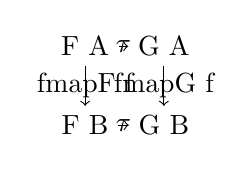
\begin{tikzpicture}
      \node (f a)                {\textagda{F A}};
      \node (f b) [below of=f a] {\textagda{F B}};
      \node (g a) [right of=f a] {\textagda{G A}};
      \node (g b) [below of=g a] {\textagda{G B}};

      \draw [->] (f a) to node [swap] {\textagda{fmapF f}} (f b);
      \draw [->] (g a) to node        {\textagda{fmapG f}} (g b);

      \draw [->] (f a) to node        {\textagda{$\tau$}} (g a);
      \draw [->] (f b) to node [swap] {\textagda{$\tau$}} (g b);
    \end{tikzpicture}
  \end{center}
  \caption{Naturality in Agda.}
  \label{fig:naturality-agda}
\end{figure}

\begin{example}
  [Identity]

  Module \module{Abel.Function}.
  \begin{codeagda}
    idNT : NT functorId functorId
    idNT = mkNT id (λ _ → refl)
  \end{codeagda}

  Compare with Example \ref{ex:natural-identity-haskell}.

\end{example}

\begin{example}
  \label{ex:natural-head-agda}

  Module \module{Abel.Data.List}.

  \begin{codeagda}
    head : {A : Set} → List A → Maybe A
    head []      = nothing
    head (x ∷ _) = just x
  \end{codeagda}
  \begin{codeagda}
    headNT : NT functorList functorMaybe
    headNT = mkNT head naturality
      where
        open Functor functorList renaming (fmap to fmapList)
        open Functor functorMaybe renaming (fmap to fmapMaybe)

        naturality : {A B : Set} {f : A → B} (xs : List A) →
                     (head ∘ fmapList f) xs ≡ (fmapMaybe f ∘ head) xs
        naturality []      = refl
        naturality (_ ∷ _) = refl
  \end{codeagda}

  Compare with Example \ref{ex:natural-head-haskell}.

\end{example}

\begin{example}
  \label{ex:natural-last-agda}

  Module \module{Abel.Data.List}.
  \begin{codeagda}
    last : {A : Set} → List A → Maybe A
    last []       = nothing
    last (x ∷ []) = just x
    last (_ ∷ xs) = last xs
  \end{codeagda}
  \begin{figure}[htbp]
    \begin{center}
      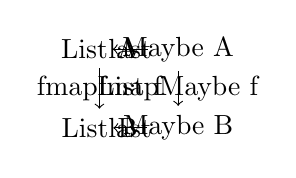
\begin{tikzpicture}
        \node (f a)                {\textagda{List A}};
        \node (f b) [below of=f a] {\textagda{List B}};
        \node (g a) [right of=f a] {\textagda{Maybe A}};
        \node (g b) [below of=g a] {\textagda{Maybe B}};

        \draw [->] (f a) to node [swap] {\textagda{fmapList f}}  (f b);
        \draw [->] (g a) to node        {\textagda{fmapMaybe f}} (g b);

        \draw [->] (f a) to node        {\textagda{last}} (g a);
        \draw [->] (f b) to node [swap] {\textagda{last}} (g b);
      \end{tikzpicture}
    \end{center}
    \caption{Naturality of the \textagda{last} natural transformation.}
    \label{fig:naturality-agda-last}
  \end{figure}
  \begin{codeagda}
    lastNT : NT functorList functorMaybe
    lastNT = mkNT last naturality
      where
        open Functor functorList renaming (fmap to fmapList)
        open Functor functorMaybe renaming (fmap to fmapMaybe)

        naturality : {A B : Set} {f : A → B} (xs : List A) →
                     (last ∘ fmapList f) xs ≡ (fmapMaybe f ∘ last) xs
        naturality []           = refl
        naturality (_ ∷ [])     = refl
        naturality (_ ∷ _ ∷ xs) = naturality (_ ∷ xs)
  \end{codeagda}

  Compare with Example \ref{ex:natural-last-agda}.

\end{example}

\section{References}
\label{sec:naturals-references}

\todo{...}

\clearemptydoublepage
